% !TEX root = ../Diplombericht.tex
\newpage
\section{Konzept} 
\label{sec:Konzept}
Das Konzept beschreibt den vorgesehenen Aufbau des Clusters und beinhaltet die Testfälle welche bei der Abnahme nach der Realisierung berücksichtigt werden müssen.

% !TEX root = ../Diplombericht.tex
\subsection{Physikalischer Überblick}
Die nachfolgende Abbildung stellt ein verinfachter Überblick der vorgesehenen Infratstruktur dar.

\begin{figure}[htb]
\centering
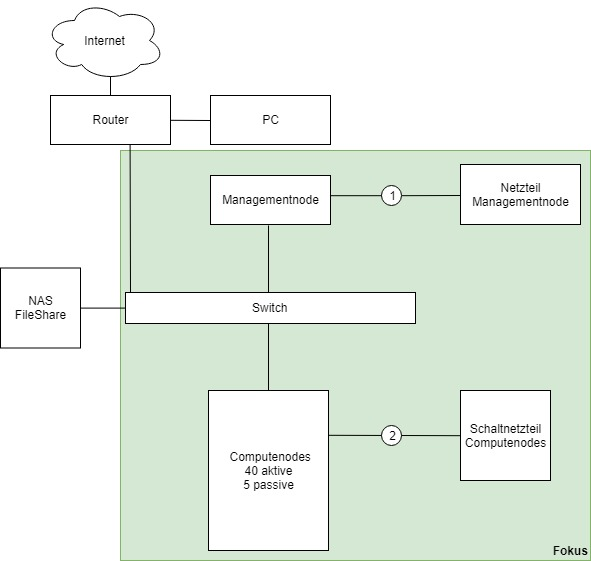
\includegraphics[scale=0.5]{phys_ueberblick.jpg}
\caption{Physikalischer Überblick}
\label{fig:Physikalischer Überblick}
\end{figure} 

\textbf{Beschreibung}\newline
Der grün markierte Teil beinhaltet das Vorhaben. Diese Komponenten werden neu in das Netzwerk eingebunden und aufgebaut. Die Komponenten ausserhalb des grünen Bereiches existieren bereits und es müssen für die Umsetzung konfigurationen vorgenommen werden.

\textbf{Verbindung 1} \newline
Der Managementnode wird über ein herkömmliches Netzteil per Micro USB mit Stom versorgt.

\textbf{Verbindung 2} \newline
Die Computenodes werden über ein Schaltnetzteil über die GPIO Pins mit Stom betrieben.



% !TEX root = ../Diplombericht.tex
\subsection{Physikalische Verbindungen}

\subsubsection{Stromversorgung Management Node}
Der Management Node wird über den Micro USB Anschluss mit Strom versorgt. Dabei muss darauf geachtet werden, dass ein mindest Strom von 2 Ampere fliesst. Zudem wird eine konstante Spannung von 5 Volt benötigt. Deshalb wird ein Netzteil mit einer Leistung von 10 Watt verwendet. Das Netzteil wird über eine Stromschiene an das Stromnetz angeschlossen.

\subsubsection{Compute Nodes}
Die Compute Nodes werden über die GPIO Pins via Jumperkabel über ein gemeinsames Netzteil mit Strom versorgt. Da es sich hierbei um eine Anzahl von mindestens 45 Raspberry's handelt, ist ein Netzteil mit einer Leistung von 500W vorgesehen. Das Netzteil wird über die Stromschiene an das Stomnetz angeschlossen.


\subsubsection{Übrige Geräte}
Die übrigen Geräte werden über den herkömmlichen Weg mit Strom über eine Stromschiene versorgt.

\subsubsection{Netzwerkverbindungen}
Die folgenden Komponenten sind über den Switch in das lokale Netzwerk eingebunden. Die nicht aufgelisteten Geräte werden direkt über Powerline oder WLAN mit dem Router verbunden:
\begin{itemize}
\item Management Node
\item Compute Nodes
\item NAS
\end{itemize}



% !TEX root = ../Diplombericht.tex
\subsection{Technischer Überblick}
\begin{figure}[H]
\centering
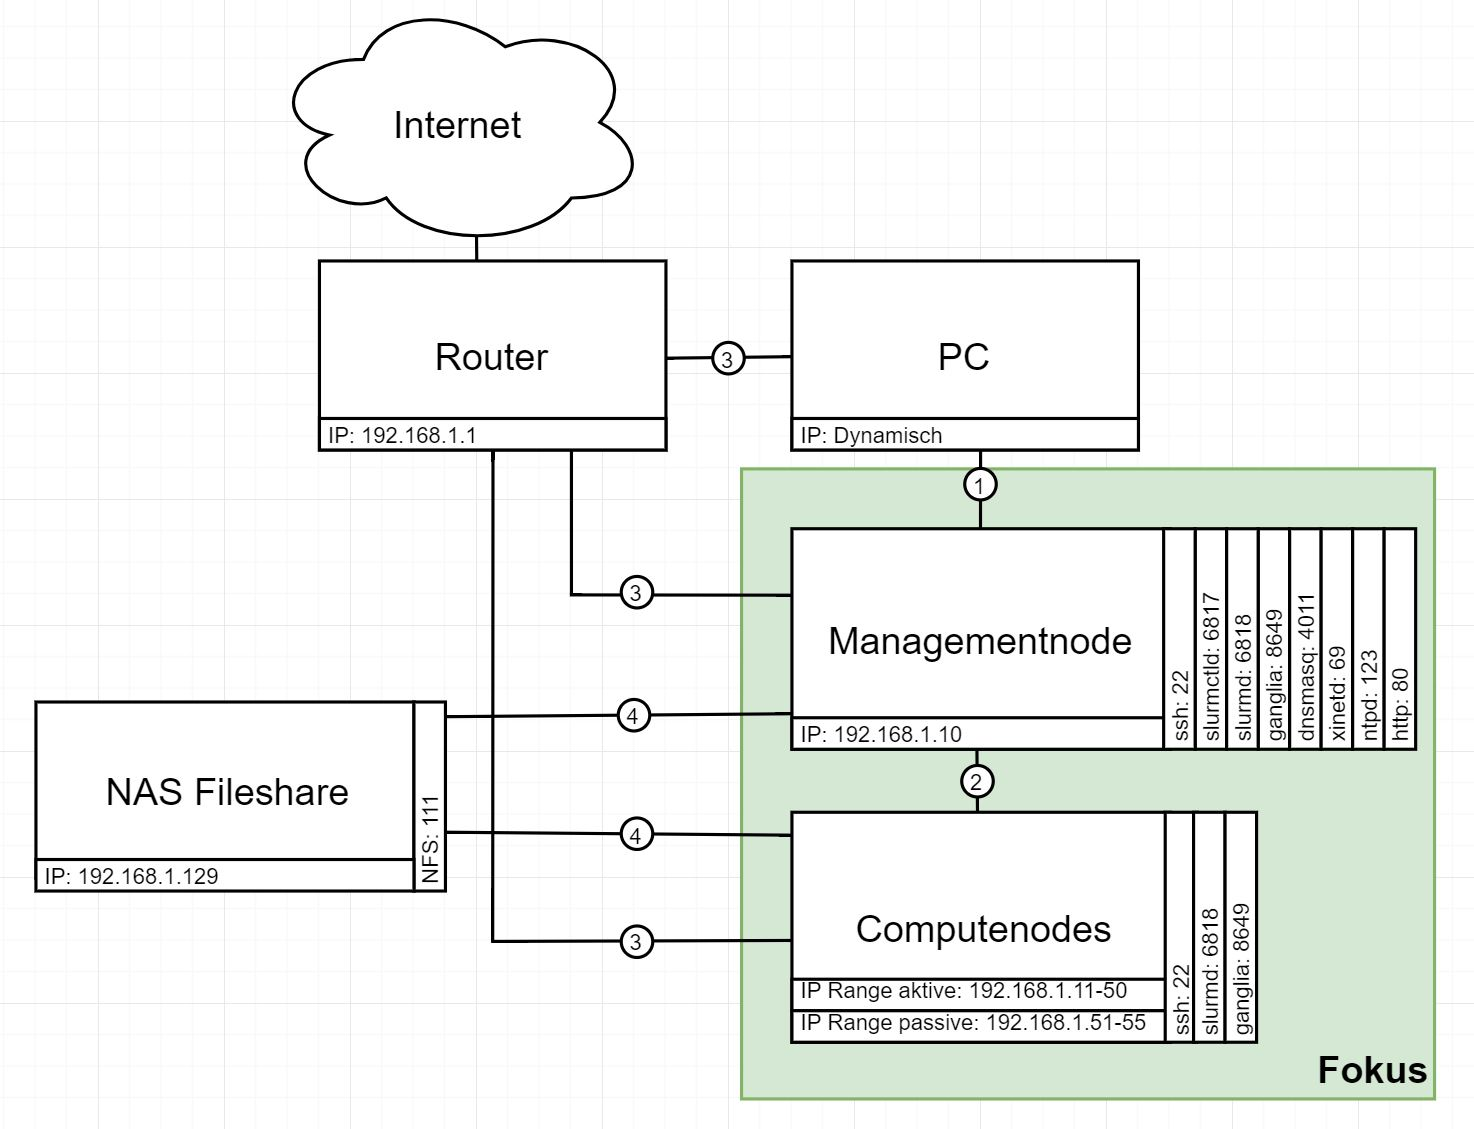
\includegraphics[scale=0.5]{tech_ueberblick.jpg}
\caption{Technischer Überblick}
\label{fig:Technischer Überblick}
\end{figure} 

\textbf{Beschreibung}\newline
Der grün markierte Teil beinhaltet das Vorhaben. Diese Komponenten werden neu in das Netzwerk eingebunden und aufgebaut. Die Komponenten ausserhalb des grünen Bereiches existieren bereits und es müssen für die Umsetzung konfigurationen vorgenommen werden.

\textbf{Verbindung 1} \newline
Der PC kann mit dem \textbf{SSH Protokoll} auf den Managementnode zugreifen. Dadurch kann die Installation vorgenommen werden. Zugleich wird über \textbf{HTTP} via Webbrowser der Zugriff auf diverse Applikationen wie z.B. Nagios \& Ganglia ermöglicht.

\textbf{Verbindung 2} \newline
Der Managementnode verteilt via \textbf{dnsmasq} und  \textbf {TFTP} das Betriebssystem an die Computenodes über das Netzwerk. Sogleich ist auch der \textbf{Slurm Controller} für die Jobsteuerung auf dem Managementnode installiert, welcher mit den \textbf{Slurm Daemons} auf den Computenodes kommuniziert. Weiterhin sind die Monitoring Komponenten \textbf{Ganglia und Nagios} auf dem Managementnode installiert, welche Monitoringdaten der Computenodes sammeln und zur Auswertung verarbeiten.

\textbf{Verbindung 3} \newline
Der Router verteilt via \textbf{DHCP} statische IP Adressen und Hostnamen welche über die MAC Adressen definiert sind.

\textbf{Verbindung 4} \newline
Der NAS Share wird über \textbf{SMB} auf den Computenodes und dem Masternode angehängt.

\subsubsection{Verwendete Protokolle}
\begin{table}[H]
\centering
\begin{tabular}{p{2cm}p{4cm}p{5cm}p{5cm}}
\hline
\rowcolor{heading} \textbf{Verbindung} & \textbf{Protokoll} & \textbf{Protokollfamilie} & \textbf{Ports} \\\hline
1 & SSH & TCP & 22 \\\hline
2 & SMTP & TCP & 25 \\\hline
3 & DHCP & UDP & 67 / 78 \\\hline
4 & TFTP & UDP & 69 \\\hline
5 & HTTP & TCP & 80 \\\hline
6 & SMB & TCP & 445 \\\hline
\end{tabular}
\caption{Protokolle}
\end{table}

% !TEX root = ../Diplombericht.tex
\subsection{Technische Verbindungen \& Kommunikation}
\begin{table}[H]
\centering
\begin{tabular}{p{1cm}p{1.5cm}p{1.5cm}p{2.2cm}p{8.8cm}}
\hline
\rowcolor{heading} \textbf{Nr.} & \textbf{Quelle} & \textbf{Ziel }& \textbf{Betrifft} & \textbf{Beschreibung} \\\hline
1 & NAS & Mgmt & Datenablage & Der NAS Share wird über das NFS Protkoll angehängt. \\\hline
2 & NAS & Compute & Datenablage & Der NAS Share wird über das NFS Protkoll angehängt. \\\hline
3 & Router & Mgmt & IP Adresse & Anhand der MAC Adresse wird eine statische IP Adresse zugewiesen. \\\hline
4 & Router & Compute & IP Adressen & Anhand der MAC Adressen werden statische IP Adressen zugewiesen. \\\hline
5 & Router & Mgmt &Hostname & Es wird über den Router ein definierter Hostname verteilt. \\\hline
6 & Router & Compute & Hostnamen & Es werden über den Router definierte Hostnamen verteilt. \\\hline
7 & Mgmt & Compute & Netzwerkboot & Der Management Node beliefert die Compute Nodes über das TFT Protokoll mit dem Betriebssystem \\\hline
8 & Internet & Mgmt & Zeitserver & Die aktuelle Zeit wird mit NTP über das Internet synchronisiert.\\\hline
9 & Mgmt & Compute & Zeitserver & Die Compute Nodes beziehen die aktuelle Zeit über NTP.\\\hline
10 & Internet & Compute & Internetzugriff & Die Compute Nodes können über ein Routing über den Mgmt auf das Internet zugreifen. \\\hline
11 & PC & Mgmt & Zugriff & Verbindungen über den PC können mit dem SSH Protokoll aufgebaut werden. \\\hline
12 & PC & Compute & Zugriff & Verbindungen über den PC können mit dem SSH Protokoll aufgebaut werden. \\\hline
\end{tabular}
\caption{Verbindungen \& Kommunikation}
\end{table}
\textbf{Legende:} Mgmt = Management Node, Compute = Compute Nodes, PC = Home Computer

% !TEX root = ../Diplombericht.tex
\subsection{Komponentenbeschreibung}
\subsubsection{Router}

Bei dem Router handelt es sich um eine Internet-Box Plus von Swisscom. Das Admin Interface ist über http://internetbox aufrufbar.

\subsubsection{PC}
Der PC ist selbst zusammengestellt und wird nur für Webzugriffe auf Applikationen welche auf dem Managementnode laufen verwendet. Zusätzlich wird per SSH auf den Managementnode zugegriffen.

\subsubsection{Managementnode}
Der Managementnode dient der Jobsteuerung sowie Clusterverwaltung. Alle zentralen Programme sind auf diesem Node installiert.

\begin{table}[H]
\centering
\begin{tabular}{|l|l|}
\hline
Hostname & nebula \\\hline
Modell & Raspberry PI 3 \\\hline
Betriebssystem & Centos 7.4 \\\hline
Architektur & 64 Bit \\\hline
\end{tabular}
\caption{Komponente Managementnode}
\end{table}

\subsubsection{Netzteil Managementnode}
Das Netzteil liefert eine konstante Spannung von 5V und Strom von mindestens 2 Ampere. Dabei handelt es sich um ein Noname Netzeil welches eine Mindestleistug von 10 Watt aufbringen muss.

\subsubsection{NAS}
Das NAS ist von der Firma Synology, das Modell lautet DS216 und wird als redundanter Datenspeicher benutzt.

\subsubsection{Switch}
Der Managed Switch TL-SL3428 von TP-Link wird für die Kommunikation zwischen NAS, Managementnode und den Computenodes benötigt. Auf die Managed Funktion wird allerdings während des Aufbaus und Betriebs verzichtet.

\subsubsection{Computenodes}
Die Computenodes erhalten über das Netzwerk das Betriebssystem durch den Managementnode zugestellt. Dabei sind alle Hostnamen mit dem Prefix "c" versehen und werden aufnummeriert. Dabei sind die Computenodes in aktiv und passiv (Fallback, Reserve) aufgeteilt, die passiven Computenodes sollen ausgefallene aktive Computenodes ersetzen und deren Arbeiten und Leistung übernehmen.

\textbf{Aktiv}
\begin{table}[H]
\centering
\begin{tabular}{|l|l|}
\hline
Hostname & c[1-40] \\\hline
Modell & Raspberry PI 3 \\\hline
Betriebssystem & Centos 7.4 \\\hline
Architektur & 64 Bit \\\hline
\end{tabular}
\caption{Komponente aktive Copmputenodes}
\end{table}

\textbf{Passiv}
\begin{table}[H]
\centering
\begin{tabular}{|l|l|}
\hline
Hostname & c[41-45] \\\hline
Modell & Raspberry PI 3 \\\hline
Betriebssystem & Centos 7.4 \\\hline
Architektur & 64 Bit \\\hline
\end{tabular}
\caption{Komponente passive Copmputenodes}
\end{table}

\subsubsection{Schaltnetzteil Computenodes}
Das Schaltnetzteil RSP-750-5 von Mean Well liefert konstante 5 Volt aus Ausgangsspannung und kann eine Leistung bis zu 500 Watt aufbringen.


% !TEX root = ../Diplombericht.tex
\subsection{Tests}
\subsubsection{Testobjekte}
Die folgende Hardware ist für die Tests der Funktionsfähigkeit des Clusters im Scope vorgesehen:
\begin{table}[H]
\centering
\begin{tabular}{p{1cm}p{7.cm}p{7.5cm}}
\hline
\rowcolor{heading} \textbf{Nr.} & \textbf{Objekt} & \textbf{Beschreibung} \\\hline
1 & Management Node & Raspberry PI 3  \\\hline
2 & Compute Nodes & Raspberry PI 3 \\\hline
3 & NAS & Synology NAS DS216 \\\hline
4 & Switch & TP-Link TL-SL3428 \\\hline
\end{tabular}
\caption{Testobjekte}
\end{table}

\subsubsection{Testarten}
Die Tests werden in folgende Kategorien eingestuft:

\begin{table}[H]
\centering
\begin{tabular}{p{1cm}p{3cm}p{12cm}}
\hline
\rowcolor{heading} \textbf{Nr.} & \textbf{Testart} & \textbf{Beschreibung} \\\hline
1 & Komponententest & Die Lauffähigkeit und Erreichbarkeit der einzelnen Hardware Komponenten wird überprüft.  \\\hline
2 & Integrationstest & Es wird die Zusammenarbeit der aktiven und neu integrierten abhängigen Komponenten überprüft. \\\hline
3 & Systemtest & Das System wird als Komplettlösung getestet. Hierbei soll geprüft werden, ob die Lösung den Anforderungen der Anwendbarkeit und Nutzbarkeit dem Auftrag entspricht.  \\\hline
\end{tabular}
\caption{Testarten}
\end{table}

\subsubsection{Testvoraussetzungen}
\textbf{Startbedingungen}\newline
Für den Start der Tests muss der Cluster aufgebaut sein und die einzelnen Komponenten müssen mit Strom versorgt sein. 

\textbf{Abbruchbedingungen}\newline
Die Tests werden abgebrochen, sobald Fehler auftauchen, welche Folgetests verhindern.

\subsubsection{Fehlerklassen}
\begin{table}[H]
\centering
\begin{tabular}{p{1cm}p{4cm}p{11cm}}
\hline
\rowcolor{heading} \textbf{Nr.} & \textbf{Fehlerklassen} & \textbf{Beschreibung} \\\hline
1 & Fehlerfrei & Die Erwartungen sind erfüllt.  \\\hline
2 & Harmloser Mangel & Es sind keine Betriebsverhinderungen zu erkennen. Die Erwartungen sind erfüllt. \\\hline
3 & Kleiner Mangel & Der Betrieb kann aufgenommen werden. Das Problem sollte aber über einen Zeitraum von 6 Monaten behoben werden.  \\\hline
4 & Schwerer Mangel & Der Cluster kann nur teilweise in Betrieb genommen werden. Der Mangel muss innerhalb zwei Wochen behoben werden. \\\hline
5 & Kritischer Mangel & Der Cluster kann nicht in Betrieb genommen werden. Die Mängel müssen umgehend behoben werden. \\\hline
\end{tabular}
\caption{Fehlerklassen}
\end{table}

\subsubsection{Testhilfsmittel}
Die Dokumentation der Tests wird im Testprotokoll nachgeführt. Damit die Tests durchgeführt werden können wird ein PC oder Notebook als Testclient benötigt. Dieser Client muss sich im selben Netzwerk wie der Cluster befinden.


% !TEX root = ../Diplombericht.tex
\subsection{Monitoring}
Es werden zwei Überwachungsapplikationen eingesetzt, welche über einen Browser aufrufbar sind. Dabei wird zwischen Service- und Performancemonitoring unterschieden.

\subsubsection{Service Monitoring}
Als Servicemonitoring wird die Applikation Nagios eingesetzt. Alle Abfragen auf sämtliche Nodes finden automatisiert vom Managementnode aus statt. Sämtliche Fehler werden per E-Mail gemeldet. Adresse gemeldetDabei müssen folgende Überwachungen implementiert werden.

\begin{table}[H]
\begin{tabular}[t]{p{0.6cm}p{2.5cm}p{2.2cm}p{1.5cm}p{8.8cm}}
\hline
\rowcolor{heading}\textbf{Nr.} & \textbf{Überwachung} & \textbf{Schweregrad} & \textbf{Intervall} &\textbf{Beschreibung} \\\hline
1 & Erreichbarkeit & Kritisch & 5 & Es wird mittels Ping eine Statusüberprüfung der Nodes durchgeführt \\\hline
2 & SSH Zugriff & Mittel & 60 & Die Zugriffe auf die Computenodes sollen über den Managementnode stattfinden  \\\hline
3 & CPU Last & Hoch & 5 & Die CPU's ständig ausgelastet sein  \\\hline
\end{tabular}
\caption{Service Monitoring}
\end{table}

\textbf{Meldungen \& Alarme} \newline
Sobald sich der Status einer Überwachung ändert, wird eine Nachricht per E-Mail an den Systemadministrator gesendet.





% !TEX root = ../Diplombericht.tex
\subsection{Hostnamen}
Die Compute Node Namen wurden nach einem überschaulichen Konzept definiert. Jeder Compute Node trägt den Prefix "c". Dies soll bei der Behebung von Problemen auf physicher Ebene, z.B. Austauschen eines Nodes, dienen. Zudem werden alle Hostnamen immer in kleinen Buchstaben geschrieben. 

\subsubsection{Management Node Name}
\begin{table}[H]
\centering
\begin{tabular}{p{5cm}p{5.5cm}p{5.5cm}}
\hline
\rowcolor{heading} \textbf{Name} & \textbf{IP} & \textbf{MAC} \\\hline
nebula & 192.168.1.10 & B8:27:EB:32:A9:1C \\\hline
\end{tabular}
\caption{Management Node Name}
\end{table}

\subsubsection{Compute Node Namen}
\begin{longtable}{p{1cm}p{2cm}p{6cm}p{6cm}}
\hline
\rowcolor{heading} \textbf{Nr.} & \textbf{Name} & \textbf{IP} & \textbf{MAC} \\\hline
01 & c1 & 192.168.1.11 & B8:27:EB:32:39:A7\\\hline
02 & c2 & 192.168.1.12 & B8:27:EB:2E:A3:D1\\\hline
03 & c3 & 192.168.1.13 & B8:27:EB:50:45:3F\\\hline
04 & c4 & 192.168.1.14 & B8:27:EB:0D:E6:25\\\hline
05 & c5 & 192.168.1.15 & B8:27:EB:3E:96:B5\\\hline
06 & c6 & 192.168.1.16 & B8:27:EB:EE:77:DA\\\hline
07 & c7 & 192.168.1.17 & B8:27:EB:21:63:E6\\\hline
08 & c8 & 192.168.1.18 & B8:27:EB:2E:2E:CC\\\hline
09 & c9 & 192.168.1.19 & B8:27:EB:17:32:96\\\hline
10 & c10 & 192.168.1.20 & B8:27:EB:B2:1C:A9\\\hline
11 & c11 & 192.168.1.21 & B8:27:EB:AF:63:1F\\\hline
12 & c12 & 192.168.1.22 & B8:27:EB:43:00:2C\\\hline
13 & c13 & 192.168.1.23 & B8:27:EB:13:7B:18\\\hline
14 & c14 & 192.168.1.24 & B8:27:EB:43:CD:29\\\hline
15 & c15 & 192.168.1.25 & B8:27:EB:FF:C7:56\\\hline
16 & c16 & 192.168.1.26 & B8:27:EB:CE:98:66\\\hline
17 & c17 & 192.168.1.27 & B8:27:EB:5D:63:34\\\hline
18 & c18 & 192.168.1.28 & B8:27:EB:91:3E:0F\\\hline
19 & c19 & 192.168.1.29 & B8:27:EB:F4:65:EC\\\hline
20 & c20 & 192.168.1.30 & B8:27:EB:3E:AB:DC\\\hline
21 & c21 & 192.168.1.31 & B8:27:EB:66:60:F6\\\hline
22 & c22 & 192.168.1.32 & B8:27:EB:37:3F:74\\\hline
23 & c23 & 192.168.1.33 & B8:27:EB:18:5E:F0\\\hline
24 & c24 & 192.168.1.34 & B8:27:EB:B0:23:B8\\\hline
25 & c25 & 192.168.1.35 & B8:27:EB:BE:C4:94\\\hline
26 & c26 & 192.168.1.36 & B8:27:EB:FB:FF:57\\\hline
27 & c27 & 192.168.1.37 & B8:27:EB:4E:EC:CE\\\hline
28 & c28 & 192.168.1.38 & B8:27:EB:43:1C:35\\\hline
29 & c29 & 192.168.1.39 & B8:27:EB:DC:74:5F\\\hline
30 & c30 & 192.168.1.40 & B8:27:EB:D1:DE:2F\\\hline
31 & c31 & 192.168.1.41 & B8:27:EB:5E:90:34\\\hline
32 & c32 & 192.168.1.42 & B8:27:EB:DE:80:24\\\hline
33 & c33 & 192.168.1.43 & B8:27:EB:A4:79:6F\\\hline
34 & c34 & 192.168.1.44 & B8:27:EB:0A:4D:C7\\\hline
35 & c35 & 192.168.1.45 & B8:27:EB:5C:53:5F\\\hline
36 & c36 & 192.168.1.46 & B8:27:EB:F7:AF:C2\\\hline
37 & c37 & 192.168.1.47 & B8:27:EB:CE:BA:ED\\\hline
38 & c38 & 192.168.1.48 & B8:27:EB:59:38:3C\\\hline
39 & c39 & 192.168.1.49 & B8:27:EB:99:BB:8E\\\hline
40 & c40 & 192.168.1.50 & B8:27:EB:8F:7A:0D\\\hline
\caption{Compute Node Namen}
\end{longtable}


\subsubsection{Reserve Node Name}
Die Reservenodes sind als Fallback für ausgefallene Compute Nodes vorgesehen.
\begin{table}[H]
\centering
\begin{tabular}{p{1cm}p{2cm}p{6cm}p{6cm}}
\hline
\rowcolor{heading} \textbf{Nr.} & \textbf{Name} & \textbf{IP} & \textbf{MAC} \\\hline
1 & c41 & 192.168.1.51 & B8:27:EB:DE:C9:69 \\\hline
2 & c42 & 192.168.1.52 & B8:27:EB:7E:6F:48 \\\hline
3 & c43 & 192.168.1.53 & B8:27:EB:5D:DD:FE \\\hline
4 & c44 & 192.168.1.54 & B8:27:EB:A6:6D:4D \\\hline
5 & c45 & 192.168.1.55 & B8:27:EB:0C:63:10 \\\hline
\end{tabular}
\caption{Reserve Node Namen}
\end{table}